\section{Adaptive Parameter Identification}

\begin{frame}[t]{Adaptive Identification, Overview}%{LS Model Identification}

   \begin{columns}
      \column{.40\textwidth}
 %   \begin{center}
      \begin{figure}[t!]
        \begin{center}
          \includegraphics[width=\textwidth]{./pres/images/justSentry}
        \end{center}
      \end{figure}
%    \end{center}
  \column{.60\textwidth}

   \begin{itemize}
\item \alert<7>{Standard Model for Underwater Vehicle Dynamics}
\item<1-6> 3-DOF Rotational Dynamics Adaptive Identification (AID) Stability Analysis
\item<1-6> 6-DOF UV AID Algorithm
\item<1-6> Experimental Evaluation: 6-DOF UV AID
   \end{itemize}
\end{columns}
\vskip9pt
\alt<1-4>{
\pause
Previous Research into UV Parameter Identification:
\pause
\begin{itemize}
\item Most previously reported studies used conventional least squares identification (LS).
\begin{itemize}
\item LS requires UV acceleration to be instrumented; this signal is
  frequently not instrumented.
\end{itemize}
\pause
\item Previously reported adaptive methods were Adaptive Model-Based
  Controllers (AMBCs). These are not applicable when
\begin{itemize}
\item UV is uncontrolled,
\item under open-loop control, or
\item using any control law other than a specific trajectory-tracking AMBC.
\end{itemize}
\end{itemize}}
{
\uncover<5-6>{
\begin{itemize}
 \item<5-6> Adaptive identification algorithms do not require simultaneous
    reference trajectory-tracking control, nor do they require
    instrumentation of linear acceleration or angular acceleration;
  \item<6> Together, these facts make adaptive identification applicable
    to a wider class of UVs than previously reported methods.
  \end{itemize}
}
}
\end{frame}


\subsection{Standard Underwater Vehicle (UV) Model}

\begin{frame}[t]{Standard Underwater Vehicle (UV) Model}%{LS Model Identification}
 \begin{align} 
   \dot{H}(t)&=\underbrace{H(t)\widehat{v(t)}}_{\text{Kinematics}}
   \nonumber \\
   \underbrace{M\dot{v}(t)}_{\text{Inertial}}&=\underbrace{\ad_{v(t)}^TM v(t)}_{\text{Coriolis}}
   +\underbrace{\sum_{i=1}^6 |v_i |D_i v(t)}_{\text{Drag}} 
   +\underbrace{\mathcal{G}(g,b,H(t))}_{\text{Gravitational}}
   +\underbrace{u(t)}_{\text{Input}}
   \nonumber
\end{align}

\end{frame}


\begin{frame}[t]{Standard Underwater Vehicle (UV) Model}%{LS Model Identification}
 \begin{align} 
   \dot{H}(t)&={\color<3>{cyan}H(t)}\widehat{\color<3>{cyan} v(t)}
   \nonumber \\
   \alert<4-5>{M}\dot{v}(t)&=\ad_{\color<3>{cyan} v(t)}^T\alert<4-5>{M}{\color<3>{cyan} v(t)}  +
   \sum_{i=1}^6 |{\color<3>{cyan}v_i} |\alert<4-5>{D_i}
            {\color<3>{cyan}v(t)}+
   \mathcal{G}(\alert<4-5>{g},\alert<4-5>{b},{\color<3>{cyan}H(t)})+\color<2>{green}u(t)
   \nonumber 
 \end{align}


 \alt<1-4>{ 
    \begin{columns}
      \column{.55\textwidth}
      \pause
 %     \pause
      \color<2>{green}{Plant Input}
      
      \begin{itemize}
      \item
        ${\color<2>{green}u(t)}\in \mathbb{R}^6$ control force and torque
      \end{itemize}

      \vskip5pt plus.5fill

      \pause

      \color<3>{cyan}{Plant States}
      
      \begin{itemize}
      \item
        ${\color<3>{cyan}H(t)}\in \SE3$ pose

        (position and orientation)
      \item
        ${\color<3>{cyan}v(t)}\in \mathbb{R}^6$  velocity

        (body frame translational and angular velocities)
      \end{itemize}

      \column{.45\textwidth}


      

     \pause 
     \alert<4>{Parameters} (241 scalar parameters)
      \begin{itemize}
      \item
        ${\alert<4> M}\in \mathbb{R}^{6\times 6}$ sum of vehicle and
        hydrodynamic mass 
        
        (21 scalar parameters)
      \item
        $\alert<4>{D_i}\in \mathbb{R}^{6\times 6}$ Drag 
        
        (216 scalar parameters)  
      \item
        ${\alert<4> b}\in \mathbb{R}^{3}$ Buoyancy torque 
        
        (3 scalar parameters)
      \item
        ${\alert<4> g}\in \mathbb{R}$ Gravitational force 
        
        
        (1 scalar parameter)
      \end{itemize}

    \end{columns} 
  }
  {
    \begin{itemize}
    \item<5-> Parameters enter linearly into UV Model
      % \item<9-> $W:\mathbb{R}^3\times\mathbb{R}^3\times\SE3
      %   \to\mathbb{R}^{36\times 3}$ is a regressor matrix
    \item<6-> LS estimate of parameters possible, requires signals 
      $\{\dot{v}(t),v(t),H(t),u(t)\}$
    \item<7-> vehicle acceleration, $\dot{v}(t)$, is typically not instrumented  
    \item<8-> Adaptive Identification does not require $\dot{v}(t)$
    \end{itemize}
  }

\end{frame}



%\subsection{Rotating Rigid Body Model}

\begin{frame}[t]{A Simpler Model\dots Rotating Rigid Body}%{LS Model Identification}

Standard Underwater Vehicle (UV) Model
  
  \begin{align} 
   \dot{H}(t)&=\underbrace{H(t)\widehat{v(t)}}_{\text{Kinematics}}
   \nonumber \\
   \underbrace{M\dot{v}(t)}_{\text{Inertial}}&=
   \underbrace{\ad_{v(t)}^TM v(t)}_{\text{Coriolis}}
   \uncover<1>{+\underbrace{\sum_{i=1}^6 |v_i |D_i v(t)}_{\text{Drag}} 
   +\underbrace{\mathcal{G}(g,b,H(t))}_{\text{Gravitational}}}
   +\underbrace{u(t)}_{\text{Input}}
   \nonumber
\end{align}
\pause

Rotating Rigid Body Model

\begin{align} 
    \dot{R}(t)&=\underbrace{R(t)\mathcal{J}(\omega(t))}_{\text{Kinematics}}
    \nonumber \\
    \underbrace{I\dot{\omega}(t)}_{\text{Inertial}}&=\underbrace{\mathcal{J}(I\omega(t))\omega(t)}_{\text{Coriolis}}
    +\underbrace{\tau(t)}_{\text{Input}}
    \nonumber
  \end{align}

  \pause
  
            {\tiny  
                 C. J. McFarland and L. L. Whitcomb. A New Adaptive
                Identifier for Second-Order Rotational Plants with
                 Applications to Underwater Vehicles.  In OCEANS,
                   2012. Proceedings of MTS/IEEE, pages 1-9, Hampton
                 Roads, VA, 2012}


\end{frame}


%\begin{frame}[t]{Rigid Body Model}
%  \begin{align} 
%    \uncover<1>{\dot{R}(t)}&\uncover<1>{=R(t)\mathcal{J}(\omega(t))}
%    \nonumber \\
%    I\dot{\omega}(t)&=\mathcal{J}(I\omega(t))\omega(t)
%    \uncover<1>{+\left(\sum_{i=1}^3 |\omega_i|C_i
%    \right)\omega(t)+\mathcal{J}(b)R(t)^T e_3}+u(t)
%    \nonumber 
% \end{align}
%
% \begin{itemize}
%   \item<2-> Standard Second Order Rotating Rigid Body System 
%   \item<3-> Typically used to model satellites
%   \item<4-> We first developed an Adaptive Identifier for this system first
% \end{itemize}
%
%\end{frame}


%\begin{frame}[t]{Rotating Rigid Body Model}%{LS Model Identification}
%  Second-Order Rotational Plant Model
%  
%  \begin{align} 
%    \dot{R}(t)&=\underbrace{R(t)\mathcal{J}(\omega(t))}_{\text{Kinematics}}
%    \nonumber \\
%    \underbrace{I\dot{\omega}(t)}_{\text{Inertial}}&=\underbrace{\mathcal{J}(I\omega(t))\omega(t)}_{\text{Coriolis}}
%    +\underbrace{\tau(t)}_{\text{Input}}
%    \nonumber
%  \end{align}
%
%  
%
%\uncover<2->{
%  \begin{columns}
%  \column{.45\textwidth}
%\begin{itemize}
%  \item  $I\in\mathbb{R}^{3 \times 3}$ Positive Definite Symmetric Moment of Inertia
%  \item  $\omega\in\mathbb{R}^{3}$ Angular Velocity
%\end{itemize}
%
%\column{.55\textwidth}
%
%\begin{equation*}
%\mathcal{J}\left(
%\left[ \begin{array}{c} 
%\omega_1 \\\omega_2  \\ \omega_3 \\
%\end{array} \right]\right) =
%\left[ \begin{array}{ccc}
%     0     & -\omega_3 &  \omega_2                               \\
%   \omega_3  &    0    & -\omega_1                               \\
%  -\omega_2  &  \omega_1 &    0                                  \\
%\end{array} \right]
%\end{equation*}
%\end{columns}
%}
%
%\end{frame}

\begin{frame}[t]{Rotating Rigid Body Model}%{LS Model Identification}
  
  \begin{align} 
    \dot{R}(t)&={\color<2->{cyan} R(t)}\mathcal{J}({\color<2->{cyan} \omega(t)})
    \nonumber \\
    {\alert<2-> I}\dot{\omega}(t)&=\mathcal{J}({\alert<2-> I}{\color<2->{cyan} \omega(t)}){\color<2->{cyan} \omega(t)}
    +{\color<2->{green} \tau(t)}
    \nonumber
  \end{align}



  \uncover<2->{
    \begin{columns}


      \column{.5\textwidth}
      \color<2->{green}{Plant Input}

      \begin{itemize}
        \item
          ${\color<2->{green}\tau(t)}\in \mathbb{R}^3$ control torque
      \end{itemize}

      \vskip5pt plus.5fill


      \color<2->{cyan}{Plant States}

      \begin{itemize}
        \item
          ${\color<2->{cyan}R(t)}\in \SO3$ Angular Position

        \item
          ${\color<2->{cyan}\omega (t)}\in \mathbb{R}^3$  Body Frame Angular Velocity

      \end{itemize}

      \column{.5\textwidth}




      \alert<2->{Parameters} (6 scalar parameters)
      \begin{itemize}
        \item
          ${\alert<2-> I}\in \mathbb{R}^{3\times 3}$  Inertia Tensor 

          Positive Definite Symmetric (PDS)
      \end{itemize}

    \end{columns}


    \uncover<3->{
      \begin{equation*}
        \mathcal{J}\left(
        \left[ \begin{array}{c} 
            \omega_1 \\\omega_2  \\ \omega_3 \\
        \end{array} \right]\right) =
        \left[ \begin{array}{ccc}
            0     & -\omega_3 &  \omega_2                               \\
            \omega_3  &    0    & -\omega_1                               \\
            -\omega_2  &  \omega_1 &    0                                  \\
        \end{array} \right]
      \end{equation*}}
    }

\end{frame}
\subsection{Adaptive Identification}

%\subsection{Rotating Rigid Body AID Stability Analysis}

\begin{frame}{Rotating Rigid Body Adaptive Identification Stability Analysis}

  \begin{columns}
    \column{.32\textwidth}

    
    Plant:
    \begin{equation*}
      \dot{\omega} =I^{-1}\left(\mathcal{J}(I\omega)\omega+\tau\right) 
    \end{equation*}
    
%    Identifier Equations:
%    \begin{align}
%      \dot{\hat{\omega}}=&\hat{I}^{-1}\left(
%        \mathcal{J}(\hat{I}\omega)\omega
%        + u\right) - a \Delta \omega    \nonumber \\
%      \dot{\hat{I}}=&-\frac{1}{2}\left(\zeta_1 \omega^T +\omega
%        \zeta_1^T\right)
%      \nonumber \\
%      &+\frac{1}{2}\left(\Delta\omega \zeta_2^T+\zeta_2
%        \Delta\omega^T\right)\only<5>{.}  \nonumber
%    \end{align}
    
    Adaptive Identifier:
    \begin{equation*}
      \dot{\hat{\omega}}=\hat{I}^{-1}\left(
        \mathcal{J}(\hat{I}\omega)\omega
        + \tau\right) - a \Delta \omega   
    \end{equation*}
 
   Error Coordinates:
    \begin{align}
      \Delta\omega(t)&=\hat{\omega}(t)-\omega(t)  \nonumber \\
      \Delta I(t)&=\hat{I}(t) - I                 \nonumber
    \end{align}
 
     
    Adaptive Parameter Update Law:
    \begin{align}
        \dot{\hat{I}}=&-\frac{1}{2}\left(\zeta_1 \omega^T +\omega
        \zeta_1^T\right)
      \nonumber \\
      &+\frac{1}{2}\left(\Delta\omega \zeta_2^T+\zeta_2
        \Delta\omega^T\right)\only<5>{.}
        \nonumber
    \end{align}
    

    
    \column{.68\textwidth}
    \temporal<3>
    {using these definitions:
      \begin{itemize}
      \item $\zeta_1=\mathcal{J}(\omega)\Delta \omega$
      \item
        $\zeta_2=\hat{I}^{-1}\left(\mathcal{J}\left(\hat{I}\omega\right)
          \omega +\tau\right)$
      \end{itemize}
    \pause
      and these constraints:
      \begin{itemize}
      \item $\tau(t)$ and $\omega(t)$ bounded by assumption
      \item $a\in\mathbb{R}_+$
      \item $\hat{I}(t_0)$ is SPD
      \item $\hat{\omega}(t_0)=\omega(t_0)$
      \item $\exists \epsilon \in \mathbb{R}_+$ such that $\|\Delta
        I(t_0)\|_F+\epsilon \leq min(eig(I))$
      \end{itemize}
      
    }{ 
      
      %\color{green}{Lyapunov Stability Proof Outline}
      %Lyapunov Stability Proof Outline
      Error Dynamics:
      \begin{align}
        \dot{\Delta I}&=-\frac{1}{2}\left(\zeta_1 \omega^T +\omega
          \zeta_1^T -\Delta\omega \zeta_2^T-\zeta_2 \Delta\omega^T\right)
        \nonumber \\
        \dot{\Delta \omega}&=-I^{-1}\left(a I
          \Delta\omega+\mathcal{J}(\omega)\Delta I \omega +\Delta I
          \zeta_2\right) 
        \nonumber
      \end{align}

      Lyapunov Function:
      \begin{align}
        V(t)&=\frac{1}{2}\left(\Delta \omega^{T} I \Delta \omega +
          \tr\left(\Delta I \Delta I^{T}\right)\right)
        \nonumber \\
        \dot{V}(t)&=-a\Delta\omega^{T}I\Delta\omega \nonumber
      \end{align}

      \begin{itemize}
      \item $V(t)$ positive definite, radially unbounded 
      %\item $V(t)$ 
      \item $V(t)=0$ $\Leftrightarrow$ $\Delta \omega=\vec{0}$,
        $\Delta I=0_{3\times 3}$
      \item $\dot{V}(t)$ negative semi-definite
      \end{itemize}
    }{ 

      With these conditions and Lyapunov stability analysis it can be
      shown that the adaptive identifier's angular velocity
      asymptotically converges to the plant's angular velocity
      (i.e. $\lim_{t\to \infty}\Delta \omega=\vec{0}$) and the
      estimated inertia tensor will converge to a constant value
      (i.e. $\lim_{t\to \infty}\Delta \dot{I}=0_{3\times3}$). These
      limits imply that \alert<5->{parameter estimates converge to
        values that provide input-output behavior identical to that of
        the actual experimental plant for the given input $\tau(t)$.}

    }
  \end{columns}
\end{frame}

\begin{frame}[t]{Adaptive Identification, Overview}%{LS Model Identification}

   \begin{columns}
      \column{.40\textwidth}
 %   \begin{center}
      \begin{figure}[t!]
        \begin{center}
          \includegraphics[width=\textwidth]{./pres/images/justSentry}
        \end{center}
      \end{figure}
%    \end{center}
  \column{.60\textwidth}

   \begin{itemize}
\item<1>Standard Model for Underwater Vehicle Dynamics
\item<1> 3-DOF Rotational Dynamics Adaptive Identification (AID) Stability Analysis
\item<1-2>    \alert<2>{6-DOF UV AID Algorithm} 
\item<1,3> \alert<3>{Experimental Evaluation: 6-DOF UV AID}
   \end{itemize}
\end{columns}
\end{frame}

%\subsection{UV Adaptive Identification}

\begin{frame}{UV Adaptive Identification}

  Plant:
  \vspace*{-5mm}

  \begin{equation*}
    \dot{v}=M^{-1}\left(\ad_{v(t)}^T(M v)+\sum_{i=1}^6 |v_i|D_i
    v+\mathcal{G}(g,b,H)+u\right)
  \end{equation*}
  \vspace*{-5mm}

  Adaptive Identifier:

  \vspace*{-5mm}

  \begin{equation*}
    \dot{\hat{v}}=\hat{M}^{-1}\left( \ad_v^T\hat{M}v
    +\sum_{i=1}^6 |v_i|\hat{D}_i v+\mathcal{G}(\hat{g},\hat{b},H)
    + u\right)- a \Delta v  
  \end{equation*}

  Parameter Update Laws:


  \begin{equation*}
    \dot{\hat{M}}=-\frac{\gamma_1}{2}\left(\psi_1 v^T 
    +v \psi_1^T-\Delta v \psi_2^T-\psi_2 \Delta v^T\right) 
  \end{equation*}

  \vspace*{-5mm}

  \begin{columns}

    \column{.33\textwidth}

    \begin{equation*}
      \dot{\hat{D_i}}=-\gamma_2|v_i|\Delta v v^T
    \end{equation*}

    \column{.33\textwidth}

    \begin{equation*}
      \dot{\hat{g}}=-\gamma_3\Delta \omega^T R^T e_3
    \end{equation*}

    \column{.33\textwidth}

    \begin{equation*}
      \dot{\hat{b}}=-\gamma_4\mathcal{J}(R^T e_3)\Delta \omega
    \end{equation*}

  \end{columns} 

  \vspace*{5mm}

  
  \alert<2->{For the technical conditions stated in the thesis, I show
    the identifier's velocity converges to the plant's velocity and
    parameter estimates converge to values that provide input-output
    behavior identical to that of the true plant for the given input
    $u(t)$.}

\end{frame}

%\begin{frame}{Implementation of Identification Algorithms}
%
%\end{frame}


\subsection{Experimental Evaluation: UV AID}

%\subsection{Experimental Overview}
\begin{frame}{Experimental Facility}

  \begin{columns}
    \column{.5\textwidth}

    Facility:
    \begin{itemize}
    \item Indoor freshwater tank (7.75 m diameter and 4.25 m deep)
    \item long baseline array - provides vehicle position
    \end{itemize}
    Johns Hopkins University Remotely Operated Vehicle (JHU ROV): 
    \begin{itemize}
    \item 150 kg vehicle 
    \item six 1.5 kWh DC brushless thrusters
    \item full 6 DOF control authority
    \item State-of-the-art sensor package
    \end{itemize}

    \column{.5\textwidth}

    \begin{center}
      \begin{figure}[htbp]  
        \begin{center}
          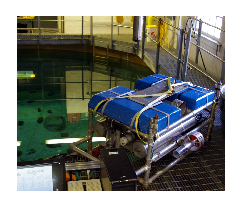
\includegraphics[width=60mm]{./appenJHUHTF/images/jhurov}
        \end{center}
        \caption{JHU ROV inside the Johns Hopkins Hydrodynamic Test
          Facility.}
      \end{figure}
    \end{center}    
  \end{columns} 
\end{frame}

%\begin{frame}
%video slide!
%\end{frame}




% \begin{frame}{Experimental Cross-Validation Method}

%     \begin{itemize}
%     \item Main idea is we performed two experiments: 
%       \begin{itemize}
%       \item First Experiment used to identify plant model (\alert<2->{IDDAT})
%       \item Second Experiment used to test identified model (\alert<2->{CROSS})
%       \end{itemize}
%     \item<3-> the input signals $u^{ID}$ and $u^{CROSS}$ were different 
%     \item<4-> In both, 3 sinusoidal moments and 3 sinusoidal force inputs 
%       were simultaneously driving the vehicle
%     \end{itemize}

%   %\begin{columns}
%   %   \column{.5\textwidth}
%   %   \begin{center}
%   %     \begin{figure}[htbp]  
%   %       \begin{center}
%   %         \includegraphics[width=50mm]{./pres/images/ID_inputSketch}
%   %       \end{center}
%   %       \caption{Identification Input}
%   %     \end{figure}
%   %   \end{center}    

%   %   \column{.5\textwidth}

%   %   \begin{center}
%   %     \begin{figure}[htbp]  
%   %       \begin{center}
%   %         \includegraphics[width=50mm]{./pres/images/CROSS_inputSketch}
%   %       \end{center}
%   %       \caption{Cross-Validation  Input}
%   %     \end{figure}
%   %   \end{center}    
%   % \end{columns} 

% \end{frame}


% \begin{frame}{Identification Algorithm Evaluation Methodology}

%   \begin{columns}
%     \column{.57\textwidth}

%     \alt<1-3> { 

%       Our goal: Evaluate if the parameter estimates of adaptive
%       identification are 'good'.

%       \pause \vskip10pt
   
%       The Straightforward Approach: Compare the parameter estimates
%       of adaptive identification to those
%       \alert<2-3>{\alt<1-2>{computed analytically}{estimated with least squares}}.

%      \vskip10pt

%      Unfortunately \alert<2-3>{\alt<1-2>{$M$, $D_1$, $D_2$, $D_3$,
%      $D_4$, $D_5$, $D_6$, $g$ and $b$ cannot be computed analytically}{
%      there is no way to guarantee that parameter sets must be 'close' to
%      one another for both to accurately model vehicle dynamics}}

%     } {

%       \alert<4-5>{Better Goal}: Evaluate if parameter estimates of
%       adaptive identification and least squares identification
%       \alert<5>{provide similar capacity to model vehicle dynamics}.

%       \vskip10pt

%       \begin{itemize}
%       \item<5-> One Experiment for identification
%       \item<6-> One Experiment for cross-validation 
%       \item<7-> Estimated model used as an Open-Loop-Observer
%       \item<8-> Plant open-loop-stable in pitch, roll, and velocity
%       \item<9-> For these DOF, use Mean Absolute Error (MAE) listed metric
%         for modeling accuracy
%       \end{itemize} 
      
%     }    
    
%     \column{.43\textwidth}
%     \only<5->{
%       \begin{center}
%         \begin{figure}[htbp]  
%           \begin{center}
%             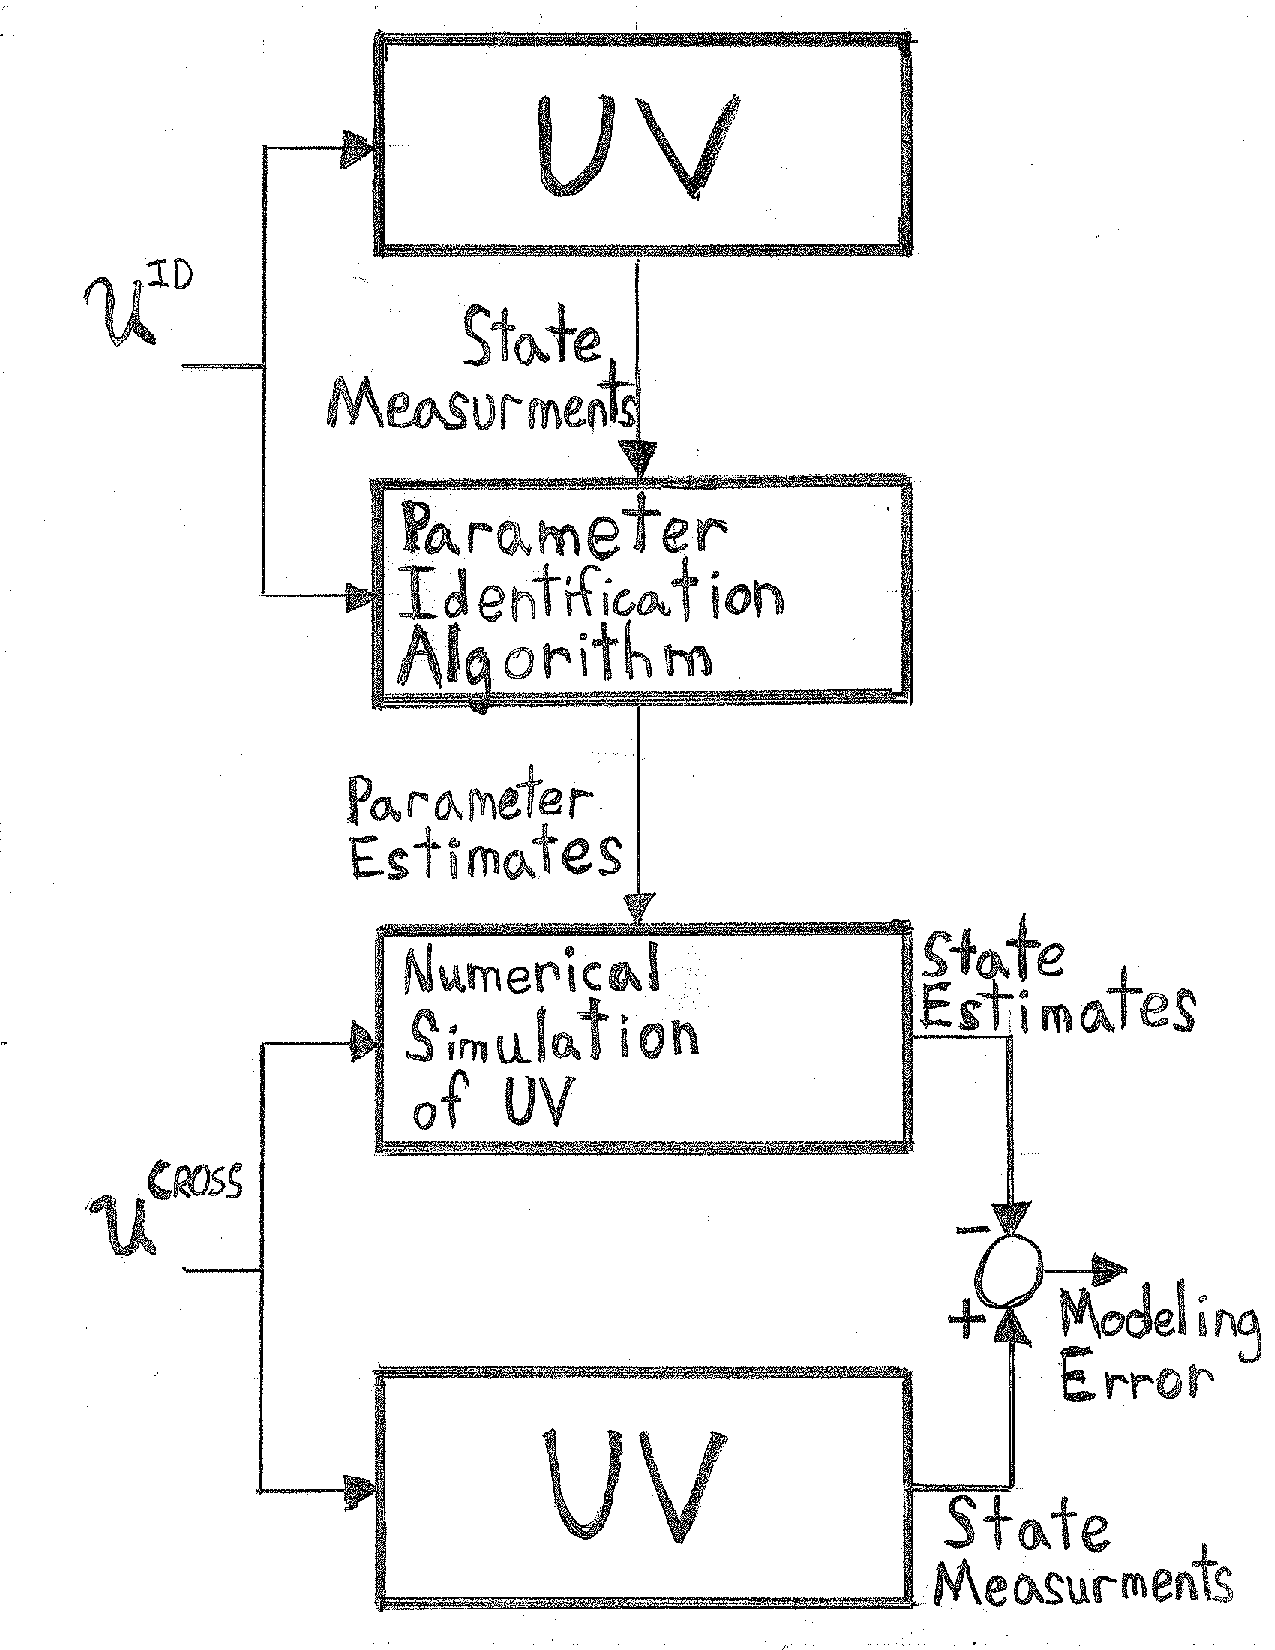
\includegraphics[width=50mm]{./pres/images/blockDiaSketch}
%           \end{center}
%         \end{figure}
%       \end{center}    

%     }  
%   \end{columns} 

% \end{frame}


\begin{frame}{Identification Algorithm Evaluation Methodology}

\begin{columns}
\column{.57\textwidth}
      \alert<1-2>{Our Goal}: Evaluate if parameter estimates of
      adaptive identification and least squares identification
      \alert<2>{provide similar capacity to model vehicle dynamics}.

      \vskip10pt

      \begin{itemize}
      \item<3-> Run two experiments 
       \begin{itemize}
       \item<3-> First experiment for parameter identification
       \item<3-> Second experiment for parameter evaluation
       \end{itemize}
     %\item<4-> Evaluation process used for \alert<6->{both Least
     %    Squares and Adaptive Identification}
     \item<3-> Compare state measurements from second experiment 
               to state estimates from UV forward simulation
      \item<3-> Mean Absolute Error (MAE) between measured and
        simulated vehicle states used to judge modeling accuracy

      \end{itemize} 
    
    \column{.43\textwidth}
     \only<3->{
      \begin{center}
        \begin{figure}[htbp]  
          \begin{center}
            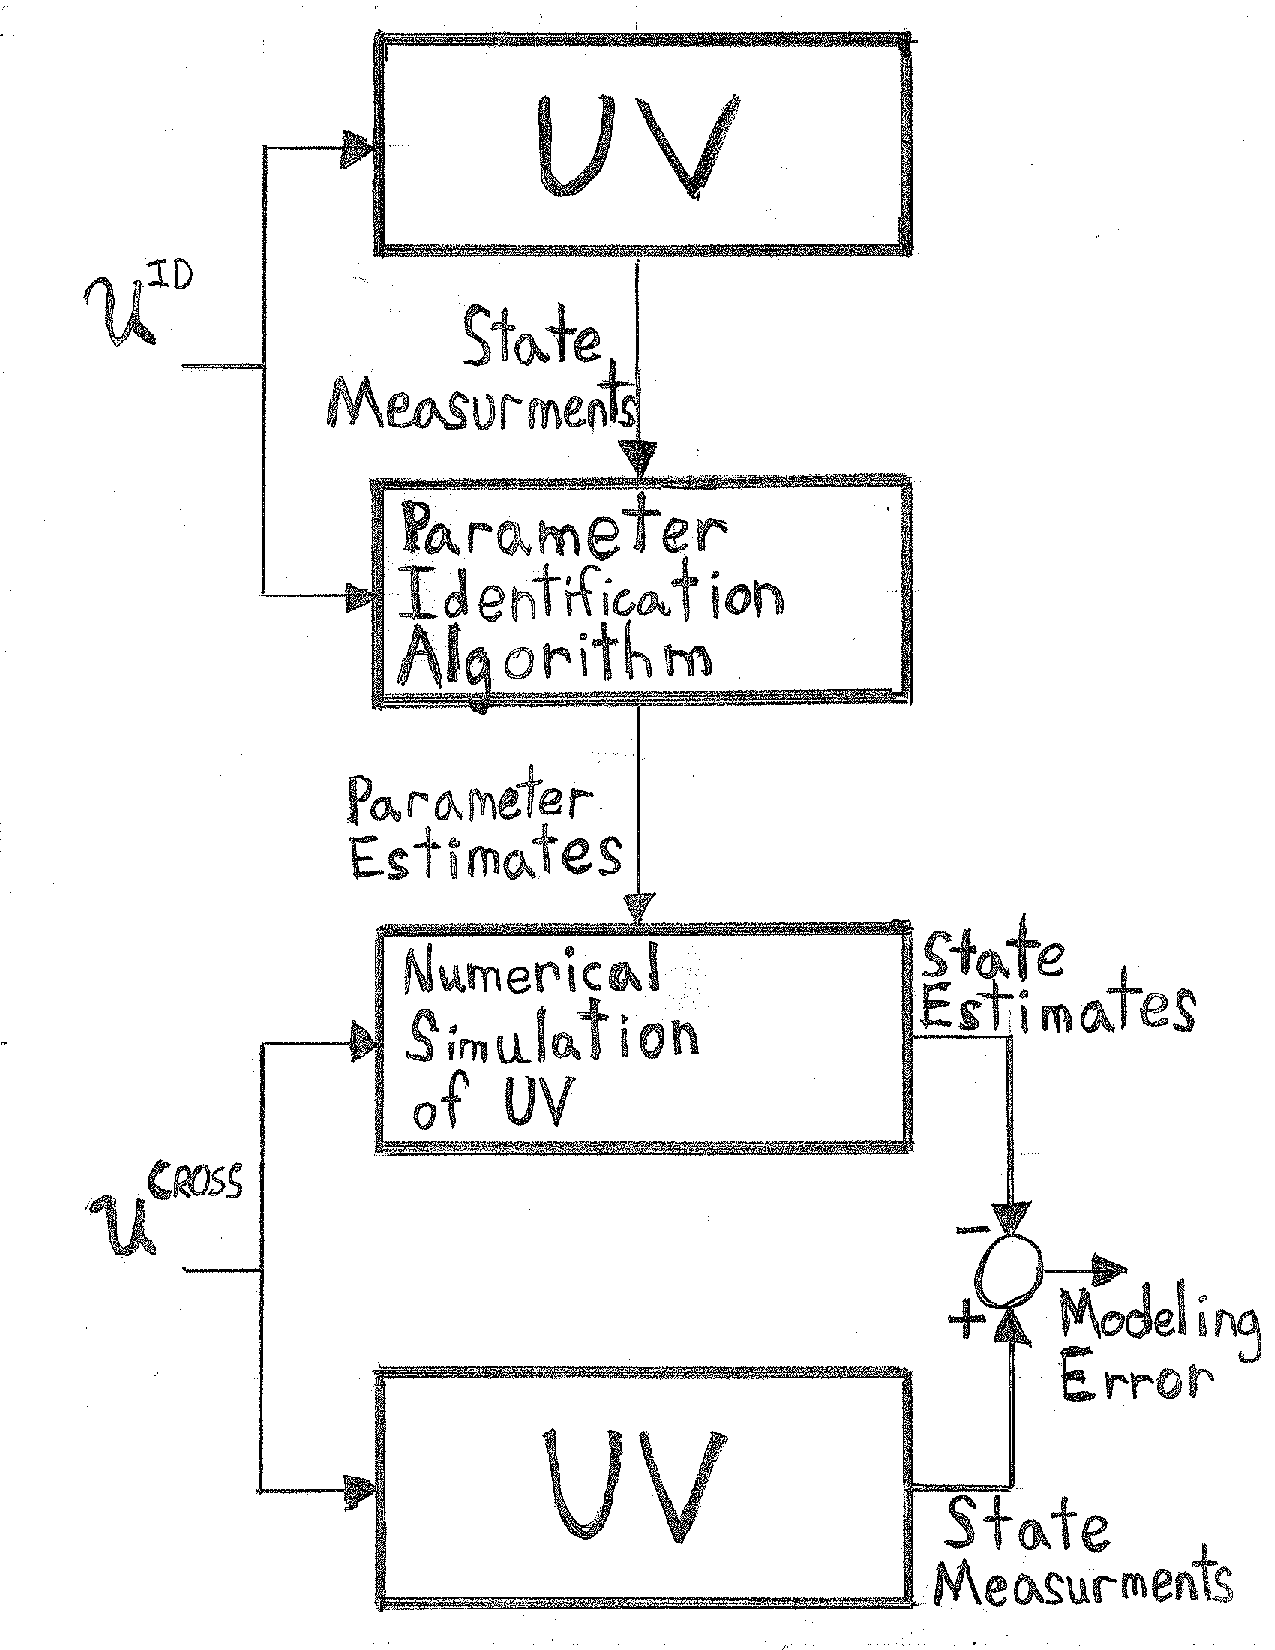
\includegraphics[width=50mm]{./pres/images/blockDiaSketch}
          \end{center}
        \end{figure}
      \end{center}    
      }
  \end{columns} 

\end{frame}

%\subsection{Cross-Validation Experiment}

\begin{frame}{Angular Position Sample Data: Roll Degree-of-Freedom}
    
    \begin{center}
      \begin{figure}[htbp]
        \begin{center}
          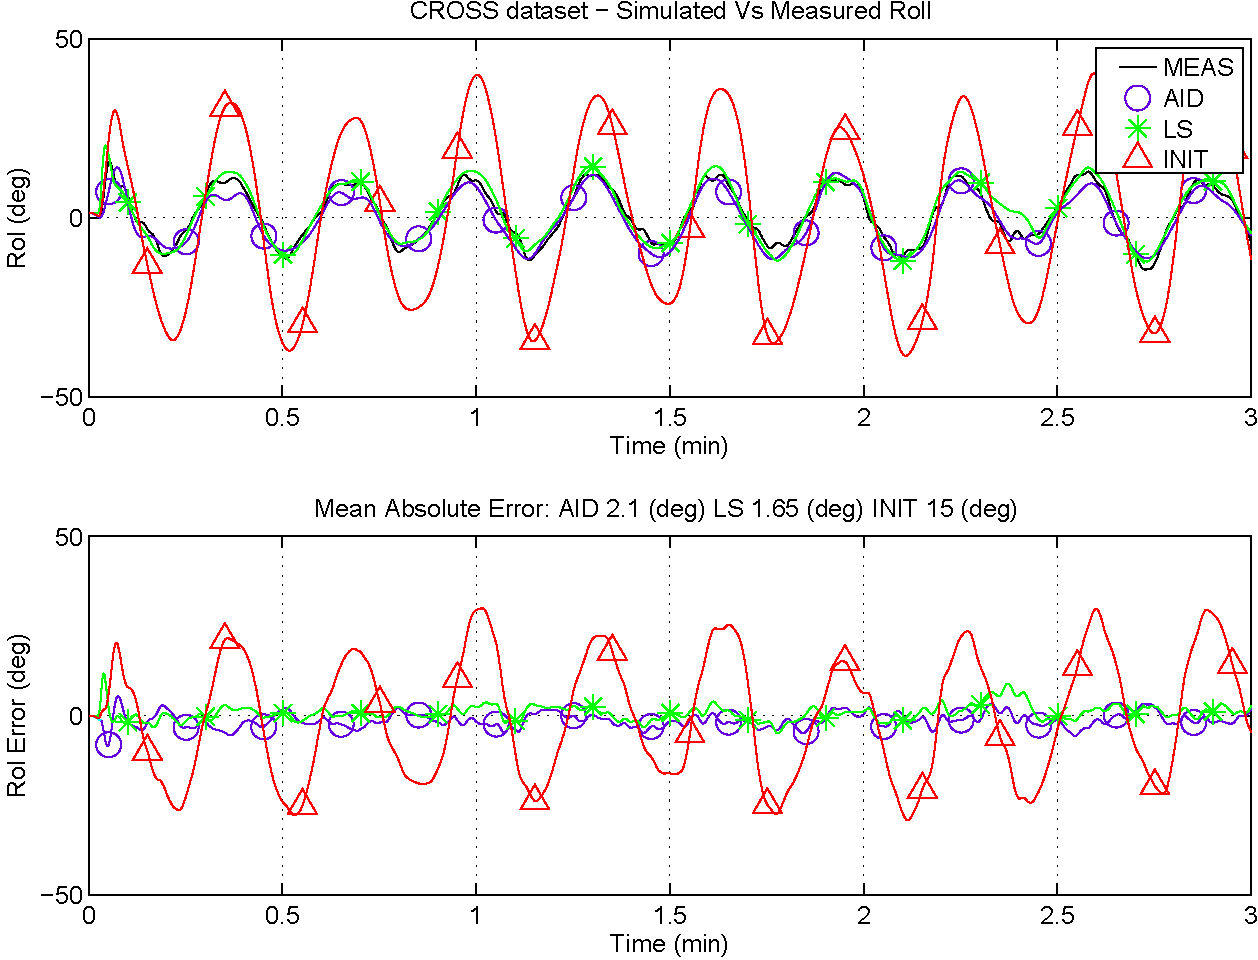
\includegraphics[width=3.5in]{./pres/images/crossALL_posExDOF_2}
        \end{center}
      \end{figure}
    \end{center}
   
\end{frame}

\begin{frame}{Analysis: Cross-Validation Experiment}

%{ \scriptsize
%\begin{table}[htbp]
%\caption{Mean Absolute Error Values for Cross-Validation Experiment}
%\begin{center}
%\begin{tabular}{p{1.5cm}|cccccccc}
% & \multicolumn{2}{c}{Angular Pose} & \multicolumn{3}{c}{Translational Velocity}& \multicolumn{3}{c}{Angular Velocity} \\ 
%Parameter Set & Roll & Pitch & x DOF & y DOF & z DOF & x DOF & y DOF & z DOF \\ \hline
%AID  &  2.0$^\circ$ & 2.1$^\circ$ & 0.062 m/s & 0.058 m/s & 0.037 m/s & 1.39$^\circ$/s & 1.35$^\circ$/s & 5.0$^\circ$/s \\
%LS   &  1.38$^\circ$ & 1.65$^\circ$ & 0.050 m/s & 0.052 m/s & 0.024 m/s & 1.38$^\circ$/s & 1.39$^\circ$/s & 6.3$^\circ$/s \\
%INIT & 9.9$^\circ$ & 15.0$^\circ$ & 0.165 m/s & 0.26 m/s & 0.25 m/s & 5.1$^\circ$/s & 3.3$^\circ$/s & 3.9$^\circ$/s \\
%\end{tabular}
%\end{center}
%\end{table}
%}
{ \scriptsize
\begin{table}[htbp]
\caption{Mean Absolute Error Values for Cross-Validation Experiment}
\begin{center}
\begin{tabular}{p{1.5cm}|cccccccc}
 & \multicolumn{2}{c}{Angular Pose ($^\circ$)} & \multicolumn{3}{c}{Translational Velocity (m/s) }& \multicolumn{3}{c}{Angular Velocity ($^\circ$/s)} \\ 
Parameter Set & Roll & Pitch & x DOF & y DOF & z DOF & x DOF & y DOF & z DOF \\ \hline
AID  &  2.0 & 2.1 & 0.062  & 0.058  & 0.037  & 1.39 & 1.35 & 5.0 \\
LS   &  1.38 & 1.65 & 0.050  & 0.052 & 0.024  & 1.38 & 1.39 & 6.3 \\
INIT & 9.9 & 15.0 & 0.165  & 0.26  & 0.25 & 5.1 & 3.3 & 3.9 \\
\end{tabular}
\end{center}
\end{table}
}
 \begin{itemize}
   \item<2-> Experimentally identified parameters model vehicle's action better 
   \item<3-> Similar modeling error by AID and LS
   \item<4-> LS might be marginally better at matching angular position
%  \item<5->
%    Adaptive Identification does not require vehicle acceleration to be instrumented
 \end{itemize}

\end{frame}


  

%\begin{frame}{Angular Velocity Sample Data: Degree-of-Freedom Y}
%    \begin{center}
%      \begin{figure}[htbp]
%        \begin{center}
%          \includegraphics[width=3.75in]{./pres/images/crossINIT_angVelExDOF}
%        \end{center}
%      \end{figure}
%    \end{center}
%    
%\end{frame}  
  
\begin{frame}{Angular Velocity Sample Data: Degree-of-Freedom Y}
    
    \begin{center}
      \begin{figure}[htbp]
        \begin{center}
          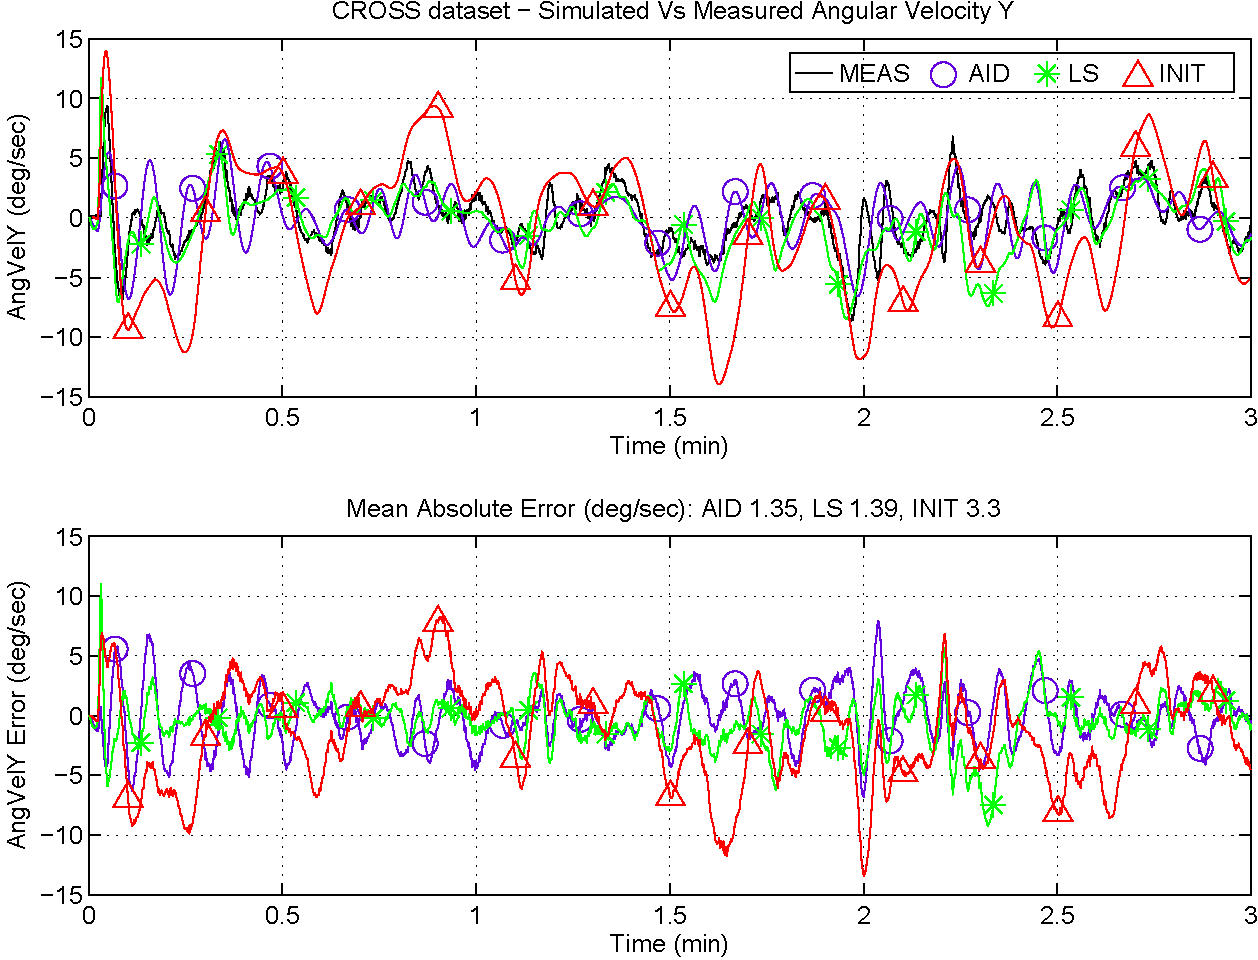
\includegraphics[width=3.75in]{./pres/images/crossAID_angVelExDOF_all}
        \end{center}
      \end{figure}
    \end{center}
   
\end{frame}


%\begin{frame}{Body Velocity Sample Data: Degree-of-Freedom Z}
%    \begin{center}
%      \begin{figure}[htbp]
%        \begin{center}
%          \includegraphics[width=3.75in]{./pres/images/crossINIT_transVelExDOF}
%        \end{center}
%      \end{figure}
%    \end{center}
    
%\end{frame}  
  
%\begin{frame}{Body Velocity Sample Data: Degree-of-Freedom Z}
%    
%    \begin{center}
%      \begin{figure}[htbp]
%        \begin{center}
%          \includegraphics[width=3.75in]{./pres/images/crossAID_transVelExDOF}
%        \end{center}
%      \end{figure}
%    \end{center}
%   
%\end{frame}


\begin{frame}{Adaptive Identification Summary}

  % Keep the summary *very short*.

   \begin{columns}
      \column{.40\textwidth}
 %   \begin{center}
      \begin{figure}[t!]
        \begin{center}
          \includegraphics[width=\textwidth]{./pres/images/justSentry}
        \end{center}
      \end{figure}
%    \end{center}
  \column{.60\textwidth}
 \begin{itemize}
  \item
    Adaptive Identification provided a good model of UV Dynamics.
  \item Least Squares and Adaptive Identification provided a similar
    capacity to model UV.
  \item Adaptive identification algorithms do not require simultaneous
    reference trajectory-tracking control, nor do they require
    instrumentation of linear acceleration or angular acceleration;
  \item Together, these facts make adaptive identification applicable
    to a wider class of UVs than previously reported methods.
  \end{itemize}
\end{columns}


  
% \pause
%  % The following outlook is optional.
%  \vskip0pt plus.5fill
%  \begin{itemize}
%  \item
%    Outlook
%    \begin{itemize}
%    \item
%      Adaptive Tracking Control for fully coupled UUV models
%    \item
%      Future directions: state observers, Coupled Adaptive Identification/Control for Fault Detection and recovery
%    \end{itemize}

\end{frame}

